\chapter{Discussion}
Please tell more about conclusion and how to the next work of this study.

\section{Aip Suprapto Munari-1164063}
\subsection{Teori}
\begin{enumerate}
\item Kenapa File Suara Harus Dilakukan Tokenizer
\begin{itemize}
\item Penjelasan: Untuk membedakan karakter-karakter tertentu dalam suatu teks dan juga sebagai pemisah kata atau bukan.Tokenizer dilakukan dengan cara melakukan pemotongan string input berdasarkan tiap kata yang menyusunnya.
\par 
\par
\item Ilustrasi Gambar
\item Tokenizer \ref{teori1}
\begin{figure}[!hbtp]
\centering
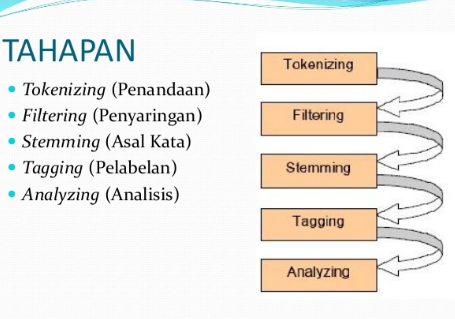
\includegraphics[scale=0.7]{figures/AIP/g1.PNG}
\caption{Tokenizer Aip}
\label{teori1}
\end{figure}
\par
\end{itemize}
\par
\par

\item 	Apa Itu Deep Learning
\begin{itemize}
\item Penjelasan: 
\par  Deep learning merupakan sub bidang pembelajaran mesin yang berkaitan dengan algoritma.
\end{itemize}
\par
\par

\item Apa itu Deep Neural Network Dan Apa Bedanya Dengan Deep Learning :
\begin{itemize}
\item Penjelasan Deep Neural Network : 
\par  Deep neural network adalah jaringan syaraf dengan tingkat kompleksitas tertentu, jaringan syaraf dengan lebih dari dua lapisan.
\par
\item Perbedaan Deep Neural Network Dan Deep Learning :
\par Perbedaan antara deep neural network dan deep learning terletak pada kedalaman model. deep learning adalah frasa yang digunakan untuk jaringan saraf yang kompleks. Kompleksitas ini disebabkan oleh pola yang rumit tentang bagaimana informasi dapat mengalir di seluruh model.
\end{itemize}
\par
\par

\end{enumerate}